\chapter{Comment faire pour ?}
\section{Générer une liste d'échantillons vides}
Objectif : préparer des bocaux d'échantillons avant de partir en campagne de collecte. Ces bocaux doivent être étiquetés.

Le logiciel propose une procédure d'import de masse, qui permet de répondre à cette question.

Voici la méthode à utiliser :
\begin{itemize}
\item générez un fichier au format CSV (créé par exemple à partir de LibreOffice OpenDataSheet -- ODS), qui comprend une ligne par échantillon ;
\item lancez la procédure d'import : le programme vous indiquera les UID générés ;
\item recherchez les UID générés, et déclenchez l'impression des étiquettes.
\end{itemize}

\subsection{Structure du fichier CSV}

Toute opération d'import présente des risques : il est difficile de revenir en arrière une fois celle-ci terminée.
Pour les limiter, le logiciel va procéder en deux étapes. D'abord, la structure du fichier va être analysée, et la cohérence des informations indiquées vérifiée.
Ensuite, si aucune anomalie n'est détectée, l'import pourra être déclenché.

La première ligne du fichier doit comporter le nom des colonnes. Leur nom est normalisé et ne doit en aucun cas être modifié. Si une colonne n'existe pas, l'import du fichier sera rejeté.

Les identifiants numériques (\textit{project\_id} par exemple) doivent être recherchés dans les tables de paramètres de l'application.

Voici la liste des colonnes utilisables :
\begin{longtable}{|p{4cm}|p{8cm}| c|}
\hline
\textbf{Colonne} & \textbf{Description} & \textbf{Obligatoire} \\
\hline
\endhead
sample\_identifier & identifiant métier de l'échantillon & X \\
\hline
project\_id & identifiant du projet de rattachement & X \\
\hline
sample\_type\_id & identifiant du type d'échantillon & X \\
\hline
sample\_status\_id & identifiant du statut à attribuer & X \\
\hline
sample\_date & date de création de l'échantillon, au format dd/mm/yyyy & \\
\hline
sample\_range & emplacement de rangement de l'échantillon dans le conteneur, si le numéro de conteneur est indiqué dans le fichier & \\
\hline
sample\_multiple\_value & nombre total (ou volume total...) de sous-échantillons associés à l'échantillon, si celui-ci est sous-échantillonnable & \\
\hline
container\_identifier & identifiant du container & X \\
\hline
container\_type\_id & identifiant du type de container & X \\
\hline
container\_status\_id & identifiant du statut à attribuer au container & \\
\hline
container\_range & emplacement de rangement du container dans son container parent & \\
\hline
container\_parent\_uid & UID du container dans lequel le container courant est rangé & \\
\hline
identifiants complémentaires & une colonne par code supplémentaire (menu \textit{Paramètres $\rightarrow$ Types d'identifiants}) & \\
\hline

\caption{Liste des colonnes utilisables lors d'un import de masse}
\end{longtable}

Les champs obligatoires ne le sont que si l'identifiant de l'objet considéré -- échantillon ou container -- a été renseigné. Une ligne doit contenir au minimum soit un numéro d'échantillon, soit un numéro de container.

\subsection{Procédure d'import}

À partir du menu, choisissez \textit{Objet $\rightarrow$ import de masse}. Seuls les utilisateurs qui disposent du droit \textit{projet} pourront réaliser l'opération.
\begin{figure}[H]
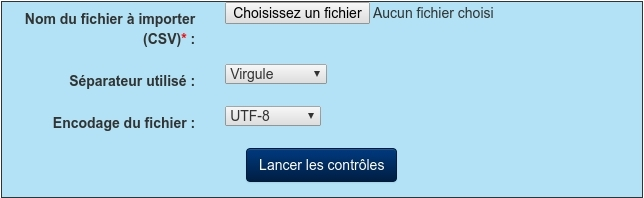
\includegraphics[width=\linewidth]{images/import_controle}
\caption{Sélection du fichier pour un import de masse}
\end{figure}

Sélectionnez le fichier à importer, vérifiez le séparateur utilisé. Préférez, si possible, les données au format UTF-8.

L'import sera réalisé ainsi :
\begin{enumerate}
\item si \textit{sample\_identifier} est renseigné : création de l'échantillon
\item si \textit{container\_identifier} est renseigné : création du container
\item si \textit{container\_parent\_uid} est renseigné : création du mouvement d'entrée du container
\item si l'échantillon et le container ont été créés, création du mouvement d'entrée de l'échantillon dans le container
\end{enumerate}

Si des anomalies sont détectées lors du contrôle, un tableau récapitulant les problèmes rencontrés sera affiché, ressemblant à ceci :
\begin{figure}[H]
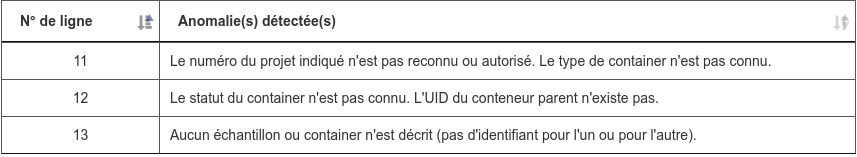
\includegraphics[width=\linewidth]{images/import_tableau}
\caption{Exemples d'anomalies détectées lors du contrôle de l'import}
\end{figure}

Si les contrôles se sont bien déroulés, le programme proposera alors de déclencher l'import, et affichera en retour les valeurs \textit{mini} et \textit{maxi} des UID générées.

\subsection{Autre usage}
Cette fonctionnalité peut également être utilisée pour déclencher l'import de listes d'échantillons pré-existants, et de créer automatiquement les mouvements adéquats pour les ranger dans leurs containers de stockage.

\subsection{Exemple de fichier}
\begin{figure}[H]
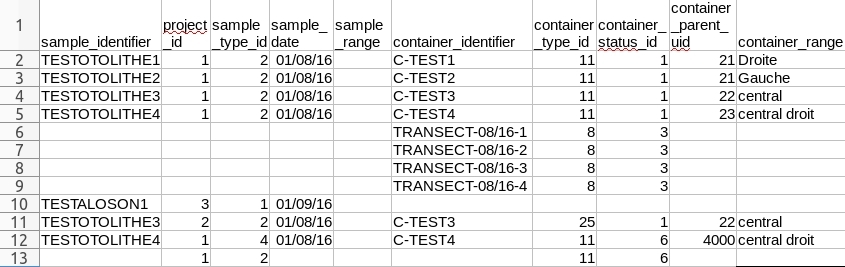
\includegraphics[width=\linewidth]{images/importcsv}
\caption{Exemple d'un fichier CSV}
\end{figure}

Dans cet exemple, l'import ne sera pas réalisé pour les raisons suivantes :
\begin{itemize}
\item en ligne 12, le numéro de container n'existe pas ;
\item la ligne 13 ne contient ni numéro d'échantillon, ni de numéro de container.
\end{itemize}

Sans tenir compte des erreurs, voici les opérations qui seraient exécutées :
\begin{itemize}
\item lignes 2 à 5, 11 et 12 : création d'échantillons, avec création du mouvement d'entrée dans les containers correspondants ;
\item lignes 6 à 9 : création de containers ;
\item ligne 10 : création d'un échantillon non rangé ;
\end{itemize}
